\documentclass[border=10pt]{standalone}
\usepackage{tikz}
\usetikzlibrary{calc,math}
\usetikzlibrary{decorations.pathmorphing}
\usetikzlibrary{decorations.markings}
\usepackage{xcolor}
\begin{document}

% if using light theme comment out below
\pagecolor{black}

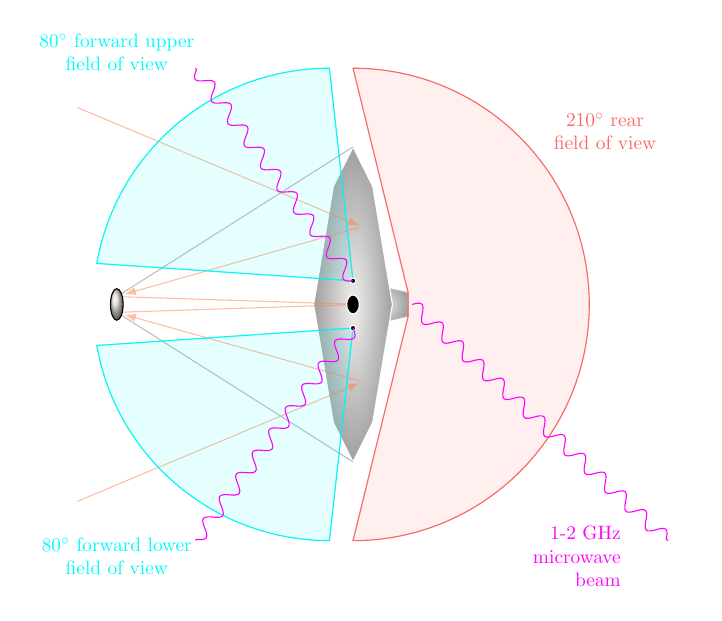
\begin{tikzpicture}[>=latex]

% colors
\definecolor{mirrorSilver}{HTML}{E5E4E2}
\definecolor{mirrorLightsilver}{HTML}{C4C4C4}
\def\mirrorShadingFill{mirrorSilver!80!mirrorLightsilver}
% it is advisable to change the mixing values
% below (60 and 70% right now) to a smaller value
% for light theme
\def\mirrorShadingOuter{mirrorSilver!70!black}
\def\mirrorShadingInner{mirrorSilver!60!white}
\def\secondaryMirrorShading{gray!10!mirrorSilver}
% background shading of the field of view shading
% it is advisable to set this to opacity=0.2 when
% using light theme
\def\fovBackgroundOpacity{0.1}

% default light theme main colors
% \def\primaryColor{black}
% \def\secondaryColor{darkgray}
% \def\bgColor{white}

% alternative dark theme colors
\def\primaryColor{white}
\def\secondaryColor{lightgray}
\def\bgColor{black}

% colors of light/light-like rays
% of course microwaves don't *actually*
% have any color, this is only for visual
% purposes
\definecolor{microwavesColor}{HTML}{FF00FF}
\definecolor{sunlightColor}{HTML}{FF7F50}

% colors of the annotated fields of view
% light theme colors
% \definecolor{customteal}{HTML}{007f7fff}
% \definecolor{customred}{HTML}{FF0000}
% alternate dark theme colors
\definecolor{customteal}{HTML}{00F9F9}
\definecolor{customred}{HTML}{FF6767}
  
\def\mirrorRadius{0.5}
\def\mirrorHeight{2}
\def\mirrorOffsetHeight{1.5}

% mirror coordinates
\coordinate (mirrorTop) at (0,\mirrorHeight);
\coordinate (mirrorBottom) at (0,-\mirrorHeight);
\coordinate (mirrorLeft) at (-\mirrorRadius,0);
\coordinate (mirrorRight) at (\mirrorRadius,0);

% laser port and spacecraft bus coordinates
\coordinate (topLaserPort) at (0,0.3);
\coordinate (bottomLaserPort) at (0,-0.3);
\coordinate (spacecraftBusTop) at (0.7,0.15);
\coordinate (spacecraftBusBottom) at (0.7,-0.15);
\coordinate (spacecraftBusBack) at (0.75,0);

% spacecraft bus
\draw[
    \secondaryColor,
    fill=\mirrorShadingFill,
    outer color=\mirrorShadingOuter,
    inner color=\mirrorShadingInner,
] (topLaserPort) -- (spacecraftBusTop) -- (spacecraftBusBottom) -- (bottomLaserPort);

% primary mirror
\draw[
    \primaryColor,
    fill=\mirrorShadingFill,
    outer color=\mirrorShadingOuter,
    inner color=\mirrorShadingInner,
] (mirrorTop) -- (-\mirrorRadius/2,\mirrorOffsetHeight) -- (mirrorLeft) -- (-\mirrorRadius/2,-\mirrorOffsetHeight) -- (mirrorBottom) -- (\mirrorRadius/2,-\mirrorOffsetHeight) -- (mirrorRight) -- (\mirrorRadius/2,\mirrorOffsetHeight) --cycle;

% incident light
\coordinate (incidentLightBouncedTop) at (-3,0.1);
\coordinate (incidentLightBouncedBottom) at (-3,-0.1);
\coordinate (incidentLightTop) at (-3.5,2.5);
\coordinate (incidentLightBottom) at (-3.5,-2.5);

% incident rays
\draw[->,sunlightColor,opacity=0.5] (incidentLightTop) -- (0.08,1);
\draw[->,sunlightColor,opacity=0.5] (0.08,0.98) -- ([shift={(0.1,0.03)}]incidentLightBouncedTop);
\draw[->,sunlightColor,opacity=0.5] (incidentLightBottom) -- (0.08,-1);
\draw[->,sunlightColor,opacity=0.5] (0.08,-0.97) -- ([shift={(0.1,-0.03)}]incidentLightBouncedBottom);

\draw[sunlightColor,opacity=0.5] (incidentLightBouncedTop) -- (0.08,0);
\draw[sunlightColor,opacity=0.5] (incidentLightBouncedBottom) -- (0.08,0);

% secondary mirror and spokes
\coordinate (secondaryMirrorAnchor) at (-3,0);
% spoke 1 
\draw[\secondaryColor] (mirrorTop) -- (-3,0.1);
% spoke 2
\draw[\secondaryColor] (mirrorBottom) -- (-3,-0.1);
% secondary mirror
\draw[ball color=\secondaryMirrorShading] (secondaryMirrorAnchor) ellipse (0.08 and 0.2);

% front field of view
\newcommand\frontFOV[3]{
    % first argument is the x-coordinate
    % of the anchor point (corresponding to
    % one of the two laser ports)
    % second is the arc's vertical height
    % third argument (1 or -1) is whether the arc will
    % face upwards (1) or downwards (-1)
    \draw[fill=customteal, opacity=\fovBackgroundOpacity] (0,#1) -- (-1*#1*#3,#2) arc[start angle=#3*90, delta angle=#3*80,radius=3cm] -- cycle;
    \draw[customteal] (0,#1) -- (-1*#1*#3,#2) arc[start angle=#3*90, delta angle=#3*80,radius=3cm, dashed] -- cycle;
}
\frontFOV{0.3}{3}{1};
\frontFOV{-0.3}{-3}{-1};

% light inlet
\draw[\primaryColor, fill=\bgColor] ellipse (0.08 and 0.12);
% front laser ports
\draw[\primaryColor, fill=\bgColor] (topLaserPort) circle (1pt);
\draw[\primaryColor, fill=\bgColor] (bottomLaserPort) circle (1pt);

% aft field of view
\draw[fill=customred,opacity=\fovBackgroundOpacity] (spacecraftBusTop) -- (0,3) arc[start angle = 90, delta angle=-180, radius=3] -- (spacecraftBusBottom) -- cycle;
\draw[customred] (spacecraftBusTop) -- (0,3) arc[start angle = 90, delta angle=-180, radius=3] -- (spacecraftBusBottom) -- cycle;

% microwave beams
\draw[microwavesColor, decorate,decoration={coil,aspect=0}] (spacecraftBusBack) -- (4,-3);
\draw[microwavesColor, decorate,decoration={coil,aspect=0}] (topLaserPort) -- (-2,3);
\draw[microwavesColor, decorate,decoration={coil,aspect=0}] (bottomLaserPort) -- (-2,-3);

% todo add the text label of the angle with "80 deg"
\node[text=customteal, text width = 3cm, scale=0.7,align=center] at (-3,3.2) {$80^\circ$ forward upper field of view};
\node[text=customteal, text width = 3cm, scale=0.7,align=center] at (-3,-3.2) {$80^\circ$ forward lower field of view};
\node[text=customred, text width = 3cm, scale=0.7,align=center] at (3.2,2.2) {$210^\circ$ rear field of view};
\node[text=microwavesColor, text width = 2cm, scale=0.7,align=right] at (2.7,-3.2) {1-2 GHz microwave beam};

\end{tikzpicture}

\end{document}
